\documentclass[12pt]{article}
\usepackage{xcolor}
\usepackage{graphicx}
%\usepackage{appendix}
%\usepackage{verbatim}
\usepackage[margin=1.0in]{geometry}
\DeclareGraphicsExtensions{.jpg,.jpeg,.png}
\renewcommand{\baselinestretch}{1.0}
\begin{document}
\newcommand{\dt}{\Delta t}
\newcommand{\Fvec}{\overline{F}}
\newcommand{\fvec}{\overline{f}}
\newcommand{\rvec}{\overline{r}}
\newcommand{\omvec}{\overline{\omega}}
\newcommand{\xvec}{\overline{x}}
\newcommand{\Xvec}{\overline{X}}
\newcommand{\yvec}{\overline{y}}
\newcommand{\Yvec}{\overline{Y}}
\newcommand{\Vvec}{\overline{V}}
\newcommand{\Rvec}{\overline{R}}
\newcommand{\Gvec}{\overline{G}}
\newcommand{\svec}{\overline{s}}
\newcommand{\Tvec}{\overline{T}}
\newcommand{\Lvec}{\overline{L}}
\newcommand{\vvec}{\overline{v}}
\newcommand{\nhat}{\hat{n}}
\newcommand{\rhvec}{\overline{\rho}}
\newcommand{\Dmat}{\overline{\overline{D}}}
\newcommand{\Rmat}{\overline{\overline{R}}}
\newcommand{\Omat}{\overline{\overline{1}}}
\newcommand{\Imat}{\overline{\overline{I}}}
\newcommand{\Hmat}{\overline{\overline{H}}}
\newcommand{\Lag}{\mathcal{L}}
\title{Simple Model of Fungal Growth on a Stationary Nutrient Medium}
\author{Written by a cast of thousands}
\maketitle

% Change table counter
\renewcommand{\thetable}{\Roman{table}}

\section{Model}
This document describes a model of fungal growth implemented with the
BoltzmannMFX framework. This model is designed to mimic the behavior of a
fungal network that is growing by elongation of tip elements and side of
segments close to the tip. Fungal elements are described as cylinders and
characterized by a length and a radius. Elements that have reached a maximum
radius only grow further by elongation.

\section{Biological Cell Dynamics}
The chemistry for this model is a fairly simple set of equations to describe
dynamics within the cell. Three chemical constituents are considered, $A$, $B$
and $C$. The cell volume is also couled to these constituents. $A$ and $C$
exist both inside and outside the cell (in the
agar medium) and the concentrations outside the cell are denoted with the
subscript $out$ and those inside the cell are labeled
with the subscript $in$. The compound $B$ is only located inside the cell.
These species are related to each other via the following reactions:
\begin{eqnarray*}
A_{out} &\stackrel{k_{1},k_{-1}}{\longleftrightarrow}& A_{in} \\
A_{in} &\stackrel{k_2,k_{-2}}{\longleftrightarrow}& B_{in} + C_{in} \\
C_{in} &\stackrel{k_3,k_{-3}}{\longleftrightarrow}& C_{out}
\end{eqnarray*}
To distinguish
between concentrations of these components and absolute amounts of component, we use
brackets [ ]. In this notation, $[A_{out}]$ is the concentration of $A$ in a grid cell and
$A_{out}$ is the total amount (mass) of $A$ in a grid cell. There is also an
additional equation that converts $B_{cell}$ into cell volume. This can be
expressed by the equation
\[
B_{in} \stackrel{k_g,k_v}{\longleftrightarrow} V_{cell}
\]
The rate constant $k_g$ describes how fast $B_{in}$ disappears from the system
and the rate constant $k_v$ describes how fast the cell volume $V_{cell}$
increases. The ratio
$k_v/k_g$ is the amount of volume that is produced by consuming a given amount
of $B_{in}$. In this model, the conversion of $B_{in}$ to volume is irreversible.

The intracellular concentration of these species is governed by the set of equations
\begin{eqnarray*}
\frac{d [A_{out}]}{d t} &=&-k_1 [A_{out}]+k_{-1} [A_{in}] \\
\frac{d [A_{in}]}{d t} &=&k_1 [A_{out}]-k_{-1} [A_{in}] - k_2 [A_{in}]
 + k_{-2}[B_{in}][C_{in}]\\
\frac{d [B_{in}]}{d t} &=&k_2 [A_{in}] - k_{-2}[B_{in}][C_{in}] - k_g[B_{in}]\\
\frac{d [C_{in}]}{d t} &=&k_2 [A_{in}] - k_{-2}[B_{in}][C_{in}]-k_{-3} [C_{in}]
+ k_3 [C_{out}] \\
\frac{d [C_{out}]}{d t} &=&k_{-3} [C_{in}]-k_3 [C_{out}]
\end{eqnarray*}
These reactions also act as sources and sinks for $A_{out}$ and $C_{out}$, which are governed
by diffusion in the agar growth medium.

An additional equation couples the concentration of $B_{in}$ to cell growth.
The growth is governed by the equation
\[
\frac{V_{cell}}{dt} = V_{cell}k_v[B_{in}]
\]
The factor of $V_{cell}$ means that the total volume produced be unit time is
governed by the total amount of $B_{in}$ insided the cell. For the time being,
the rate constants are only non-zero if the segment is below the maximum size
limits. This means that growth only occurs at growth tips or, to a lesser
extent, segments that have just branched.

The transport equations into and out of the cell can be examined in more detail.
To avoid confusion with the cell area $A_{cell}$, we focus on component $C$ but similar comments
apply to component $A$. We define coefficients $k'_3$ and $k'_{-3}$ as mass-transfer
coefficients and the fluxes of material into the cell, $f_{in}$, and out $f_{out}$ can be written
as
\begin{eqnarray*}
f_{in} &=& [C_{out}]A_{cell}k'_3 \\
f_{out} &=& [C_{in}]A_{cell}k'_{-3}
\end{eqnarray*}
where $A_{cell}$ is the surface area of the cell.
In a time increment $\dt$, the mass increments $\Delta C_{in}$ going into the cell and $\Delta
C_{out}$ going out of the cell are
\begin{eqnarray*}
\Delta C_{in} &=& \dt \frac{C_{out}}{V_{grid}}A_{cell}k'_3\\
\Delta C_{out} &=& \dt \frac{C_{in}}{V_{cell}}A_{cell}k'_{-3}
\end{eqnarray*}
Note that $C_{in}$ and $C_{out}$ are the absolute amounts of $C$ occupying a cell volume $V_{cell}$
and grid cell volume $V_{grid}$, respectively. We are ignoring possible changes in the biological
and grid cell volumes during this time interval. The incremental changes in the total amount of
material in the biological cell and the grid cells can be written as
\begin{eqnarray*}
C_{in}(t+\dt)-C_{in}(t) &=& \dt \frac{C_{out}}{V_{grid}}A_{cell}k'_3 - \dt\frac{C_{in}}{V_{cell}}
A_{cell}k'_{-3} \\
C_{out}(t+\dt)-C_{out}(t) &=& \dt \frac{C_{in}}{V_{cell}}A_{cell}k'_{-3} - \dt\frac{C_{out}}{V_{grid}}
A_{cell}k'_3
\end{eqnarray*}
Dividing the first equation $\dt V_{cell}$ and the second by $\dt V_{grid}$ and taking the limit $\dt
\rightarrow 0$ gives
\begin{eqnarray*}
\frac{d [C_{in}]}{dt} &=& [C_{out}]\frac{A_{cell}}{V_{cell}}k'_3 - [C_{in}]\frac{A_{cell}}{V_{cell}}
k'_3 \\
\frac{d[C_{out}]}{dt} &=& [C_{in}]\frac{A_{cell}}{V_{grid}}k'_{-3} - [C_{out}]\frac{A_{cell}}{V_{grid}}
k'_3
\end{eqnarray*}
Using these expressions for the change in concentration due to transport across the cell membrane, the
rate equations governing this system become
\begin{eqnarray*}
\frac{d [A_{out}]}{d t} &=&-k'_1\frac{A_{cell}}{V_{grid}} [A_{out}]
+k'_{-1}\frac{A_{cell}}{V_{grid}} [A_{in}] \\
\frac{d [A_{in}]}{d t} &=&k'_1\frac{A_{cell}}{V_{cell}} [A_{out}]
-k'_{-1}\frac{A_{cell}}{V_{cell}} [A_{in}] - k_2 [A_{in}]
 + k_{-2}[B_{in}][C_{in}]\\
\frac{d [B_{in}]}{d t} &=&k_2 [A_{in}] - k_{-2}[B_{in}][C_{in}]\\
\frac{d [C_{in}]}{d t} &=&k_2 [A_{in}] - k_{-2}[B_{in}][C_{in}]
-k'_{-3} \frac{A_{cell}}{V_{cell}}[C_{in}]
+ k'_3\frac{A_{cell}}{V_{cell}} [C_{out}] \\
\frac{d [C_{out}]}{d t} &=&k'_{-3} \frac{A_{cell}}{V_{grid}}[C_{in}]
-k'_3\frac{A_{cell}}{V_{grid}} [C_{out}]
\end{eqnarray*}
From here on in, we drop the primes on $k'_1$, $k'_{-1}$, $k'_3$ and $k'_{-3}$.

Numerically, the rate equations are currently being handled using the following scheme
\begin{list}{$\bullet$}{}
\item There is an equilibration between the fluid and the cell over a time
increment $\dt/2$
\item The internal cell reaction takes place over a time increment $\dt$
using the updated internal concentrations from the previous step
\item Using the updated internal concentrations from the reaction step, the
concentrations are re-equilibrated with the outside fluid over a time interval
$\dt/2$
\end{list}
The first step is implemented by calculating the amount of material that flows
between the biological cell and the grid cell in which it is located.
The total amount of
material that flows into the cell in the interval $\dt$ is
\begin{eqnarray*}
\Delta A & = & \frac{\dt}{2} A_{cell}(k_1 [A_{out}]-k_{-1} [A_{in}]) \\
\Delta B & = & 0 \\
\Delta C & = & \frac{\dt}{2} A_{cell}(k_3 [C_{out}]-k_{-3} [C_{in}]) \\
\end{eqnarray*}
Based on this increment, the concentrations inside and outside the cell are
adjusted using the equations
\begin{eqnarray}
\nonumber
[A'_{in}] &=& [A_{in}] + \Delta A/V_{cell} \\
\nonumber
[B'_{in}]  &=& [B_{in}] \\
\nonumber
[C'_{in}] &=& [C_{in}] + \Delta C/V_{cell}
\end{eqnarray}
\begin{eqnarray}
\nonumber
[A'_{out}] &=& [A_{out}] - \Delta A/V_{grid} \\
\nonumber
[B'_{out}]  & = & [B_{out}] \\
\nonumber
[C'_{out}] &=& [C_{out}] - \Delta C/V_{grid}
\end{eqnarray}

The second step adjusts the concentration of reactants inside the cell based on
internal chemical reactions. Using a simple Euler scheme, the adjusted values of
the concentrations after the time increment $\dt$ are
\begin{eqnarray}
\nonumber
[A'_{in}] &=& [A_{in}] + \dt(-k_2 [A_{in}] + k_{-2} [B_{in}][C_{in}]) \\
\nonumber
[B'_{in}] &=& [B_{in}] + \dt(k_2 [A_{in}] - k_{-2} [B_{in}][C_{in}]) \\
\nonumber
[C'_{in}] &=& [C_{in}] + \dt(k_2 [A_{in}] - k_{-2} [B_{in}][C_{in}])
\end{eqnarray}
After adjusting the internal concentrations using the these equations, the
concentrations inside and outside the cell are again adjusted using the
equations in the first step.

\section{Cell forces}
The cell forces are calculated using a cubic interaction as described in Mathias
{\em et al}~\cite{Mathias}. The interactions are pairwise
additive, with the force between two particles $i$ and $j$ described by a function of the form
\[
\Fvec_{ij} = F_{ij}(r_{ij})\frac{\rvec_{ij}}{r_{ij}}
\]
where $F_{ij}(r_{ij})$ is a spherically symmetric function of the separation distance between the
centers of the two particles. For this model, the function $F(r)$ has the generic form
\begin{eqnarray*}
F(r) &=& -\mu(r-R_A)^2(r-R_S)\;\;\;\mbox{if}\;\;\;r<R_A \\
& = & 0\;\;\; \mbox{otherwise}
\end{eqnarray*}
The parameter $\mu$ is the stiffness and controls the magnitude of the repulsive and attractive
interactions. $R_S$ is the equilibrium separation value at which the net force on the particles is zero
and $R_A$ is the distance at which all pair interactions vanish. For $r<R_S$, the particles repel each
other while for $R_S<r<R_A$, the particles are attracted to each other. For this model, the values of
$R_S$ and $R_A$ are functions of the individual particle radii. If particle $i$ has radius $R_i$ and
particle $j$ has radius $R_j$ then the parameter $R_S$ is chosen as
\[
R_S = R_i+R_j
\]
The width of the attractive region, $R_A-R_S$, is chosen to have a fixed value $W_A$ for all particle
interactions. The value of $R_A$ is then
\[
R_A = R_i+R_j +W_A
\]
Note that the particle radii can increase over time, so even if two particles are in mechanical
equilibrium at some time $t$, they may start pushing against each other at a later time $t'$ as they
grow.

Particles also interact with the surface of the growth medium using a similar potential. In this
the contribution to the force is only in the $z$-direction and is a function $H(z)$ of the height $z$ above
the growth medium surface. The force has the form
\begin{eqnarray*}
H(z) & = & -\xi (z-Z_A)^2(z-Z_S)\;\;\;\mbox{if}\;\;\;0<z<Z_A \\
& = & \xi Z_A^2Z_S\;\;\;\mbox{if}\;\;\;z<0 \\
& = & 0\;\;\;\mbox{otherwise}
\end{eqnarray*}
The parameter $\xi$ is the stiffness of the interaction, $Z_S$ is the equilibrium distance above the surface
and $Z_A$ is the point at which all interaction with the surface ends. Between $Z_S<z<Z_A$, particles are
attracted to the surface, while below $Z_S$ particles are repelled from the surface. Below the surface,
particles experience a constant upward force. This force is designed primarily to prevent particles from
getting accidentally pushed down into the growth medium. Similar to the pair interaction, for particle $i$,
the parameter $Z_S$ is given by
\[
Z_S = R_i
\]
and the parameter $Z_A$ is given by
\[
Z_S = R_i + W_Z
\]
where $W_Z$ is the width of the attractive region and is assumed to be independent of the particle's size.

\section{Real parameters}
It is important to come up with semi-realistic parameters for this model that
accurately reflect the time scales encountered in real systems. If we start with
hypothetical yeast system with cells that are about 1 $\mu$m in diameter, the time
to grow enough to divide once is about 40 minutes (2400 seconds). Assuming we want
to get cells to divide in about 240 steps (this is a purely arbitrary requirement)
then the desired time step is 10 seconds.

Taking glucose as
a model nutrient, the diffusion coefficient of glucose in water is $6\times 10^{-10}$
cm$^2$/sec = 600 $\mu$m$^2$/sec. The mean square displacement of a glucose molecule
in 10 seconds is
\[
\sqrt{ \frac{600\;\mu\mathrm{m}}{\mbox{sec}}\times \mbox{10 sec}}
\approx\;77\;\mu\mathrm{m}
\]
This is probably a good number for the minimal size of grid cell.

The glucose concentration can be taken as 20 mMolar. Approximately 70\% of the cell is
water. Assuming a 0.5 $\mu$m radius for the cell, the cell volume is 5.3$\times$10$^{-13}$
cm$^3$. If the cell density is approximately the same as water, then the non-water mass of
the cell is 0.3$\times$10$^{-13}$g = 1.5$\times$10$^{-13}$g. This represents
\[
1.5\times 10^{-13}\mbox{g}\times\frac{\mbox{1 mole glucose}}{180\;\mbox{g glucose}} = 8\times 10^{-16}
\mbox{mole glucose}
\]
Further assume that only 5\% of the glucose is converted to cell material, then approximately
1.6$\times$10$^{-14}$moles of glucose must be consumed to produce one cell. Given that the rate of
glucose consumption is approximately $k_2 [A_{in}]$, then amount of time required to consume this
amount of glucose is
\[
1.6\times 10^{-14}\mbox{moles} = \Delta t V_{cell}k_2 [A_{in}]
\]
If we want cells to divide about every 40 minutes then $\Delta t$ is 2400 seconds. Filling in the
remaining numbers for $V_{cell}$ and the concentration of $[A_{in}]$ gives the following value for $k_2$
\[
k_2 = 1.6\times 10^{-14}\mbox{moles}\times\frac{1}{2400\;\mbox{sec}}
\times\frac{1}{5.3\times 10^{-13}\mbox{cm}^3}
\times\frac{1}{0.02\;\mbox{moles/L}}\times\frac{10^3\mbox{cm}^3}{\mbox{L}}= 0.6\;\mbox{sec}^{-1}
\]
Based on the original value of 5.3$\times$10$^{-13}$ cm$^3$ for the cell volume, a good value for the volume
at which the cell divides is approximately twice that value, 1.0$\times$10$^{-12}$ cm$^3$.

The bimolecular coefficient $k_{-2}$ has different units that need to reflect the concentration
of species. Assume that the concentration of $[B_{in}]$ inside the cell is about 10\% of the concentration
of $[A_{in}]$ and the concentration of $C$ ia about 5\% of $[A_{in}]$. Further assume that the time scale for the
back reaction of $[A_{in}]$ is the same as the forward reaction. Then set
\[
k_2 = k_{-2}\times 0.1\times 0.05\times [A_{in}]
\]
Solving for $k_{-2}$ and substituting known values gives
\[
k_{-2} = 0.6\mbox{sec}^{-1}\times\frac{1}{ 0.005\times 0.020 \mbox{moles/L}}=6\times 10^4
\frac{\mbox{moles}}{\mbox{L sec}}
\]

We also need to calculate the coefficient $k_g$.
Ignoring the back-reaction for $B$, the rate of change of $[B_{in}]$ can be approximated as
\[
\frac{d[B_{in}]}{dt} = k_2 [A_{in}]
\]
This implies that the rate of change for the volume can be approximated as
\[
\frac{dV}{dt} = k_g V_{cell}k_2 [A_{in}]
\]
Again, assuming an interval of 40 minutes and a change of about 5.3$\times$10$^{-13}$cm$^3$, we have
\[
5.3\times 10^{-13}\mbox{cm}^3 = \Delta t k_g V_{cell}k_2 [A_{in}]
\]
Note that the left hand side is essentially $V_{cell}$, so the factors of $V_{cell}$ cancel.
Solving for $k_g$ in terms of the remaining variables and substituting the known values gives
the expression
\[
k_g = \frac{1}{2400\;\mbox{sec}} \times\frac{1}{0.6\mbox{sec}^{-1}}\times\frac{1}{0.020\;\mbox{moles/L}}
=0.035\;\mbox{L/moles}
\]

For simplicity, assume that material is transported into and out of the cell on the same time scale
that component $A$ is being consumed by the cell. This implies that
\[
k_1\frac{A_{cell}}{V_{cell}} = k_2
\]
For spherical cells of radius $r$, this expression reduces to
\[
k_1\frac{3}{r} = k_2
\]
Cells are 1.0 $\mu$m in diameter, which yields the following value for $k_1$
\[
k_1 = k_2\frac{r}{3} = \frac{1}{3}\times 0.5\times 10^{-6}\mbox{cm}\times 0.6\;\mbox{sec}^{-1}=1.0\times
10^{-7}\;\mbox{cm/sec} 
\]
This value is used for the remaining parameters $k_{-1}$, $k_3$ and $k_{-3}$.

The complete set of parameters for the system are summarized in the Calculated Value column
of the table below:

\begin{tabular}{|c|l|l|l|}
\hline
Variable & Calculated Value & Adjusted Value & Description \\
\hline
$\Delta t$ & 10 sec & 10 & Time increment \\
$\Delta x$ & 7.7$\times$10$^{-3}$ cm & 7.7$\times$10$^{-3}$ cm& Minimum grid cell dimension \\
$V_{crit}$ & 1.0$\times$10$^{-12}$ cm$^3$ & 1.0$\times$10$^{-12}$ cm$^3$
    &  Volume at which cell divides \\
$[A_{out}]_0$ & 2.0$\times$10$^{-5}$ M/cm$^3$ & 2.0$\times$10$^{-5}$ M/cm$^3$
    & Initial external concentration of $A$ \\
$[C_{out}]_0$ & 2.0$\times$10$^{-6}$ M/cm$^3$ & 2.0$\times$10$^{-6}$ M/cm$^3$
    & Initial external concentration of $C$ \\
$D_A$ & 6$\times 10^{-10}$ cm$^2$/sec & 6$\times 10^{-10}$ cm$^2$/sec & Diffusion coefficient of $A$ \\
$D_C$ & 6$\times 10^{-10}$ cm$^2$/sec & 6$\times 10^{-10}$ cm$^2$/sec & Diffusion coefficient of $C$ \\
$k_1$ & 1.0$\times$10$^{-7}$ cm/sec &\color{red}{2.0$\times$10$^{-5}$ cm/sec} & Reaction coefficient \\
$k_{-1}$ & 1.0$\times$10$^{-7}$ cm/sec &\color{red}{2.0$\times$10$^{-5}$ cm/sec} & Reaction coefficient \\
$k_2$ & 0.6 sec$^{-1}$ &\color{red}{0.4 sec$^{-1}$} & Reaction coefficient \\
$k_{-2}$ & 60 moles/(cm$^3$ sec) &\color{red}{0.06 moles/(cm$^3$ sec)} & Reaction coefficient \\
$k_3$ & 1.0$\times$10$^{-7}$ cm/sec &\color{red}{2.0$\times$10$^{-5}$ cm/sec} & Reaction coefficient \\
$k_{-3}$ & 1.0$\times$10$^{-7}$ cm/sec &\color{red}{2.0$\times$10$^{-5}$ cm/sec} & Reaction coefficient \\
$k_g$ & 35 cm$^3$/moles & 35 cm$^3$/moles & Growth rate coefficient \\
\hline
\end{tabular}

\noindent
The adjusted values are the ones that seem to work in an actual simulation. In most cases they are close
to the calculated values with the exception of $k_{-2}$. This value is substantially smaller than the
original estimate.

\section{Ellipsoidal interactions}
An ellipsoid that is centered at the origin and whose axes are aligned with the standard coordinate axes
can be written as
\[
\left(\frac{x}{a}\right)^2+\left(\frac{y}{b}\right)^2+\left(\frac{z}{c}\right)^2=1
\]
An alternative way of writing this equation is
\[
\xvec^T\cdot\Dmat\cdot\xvec=1
\]
where the matrix $\Dmat$ is diagonal
\[
\Dmat = \left[\begin{array}{ccc}
a^{-2} & 0 & 0 \\
0 & b^{-2} & 0 \\
0 & 0 & c^{-2}
\end{array}\right]
\]
If the ellipsoid is rotated by some rotation $\Rmat$ so that the axes of the ellipsoid no longer coincide
with the coordinate axes, the equation for the ellipsoid becomes
\[
\xvec^T\cdot\Rmat^{T}\cdot\Dmat\cdot\Rmat\cdot\xvec = 1
\]
Finally, if the ellipsoid is shifted from the origin and is centered at $\xvec_{0}$, the equation is
\[
(\xvec-\xvec_0)^T\cdot\Rmat^{T}\cdot\Dmat\cdot\Rmat\cdot(\xvec-\xvec_0) = 1
\]

Imagine two non-overlapping ellipsoids described by the vectors $\xvec$ and $\yvec$. We want to find the
values $\xvec'$ and $\yvec'$ that minimize the separation distance between the ellipsoid surfaces. This
is equivalent to minimizing the objective function
\[
\chi = (\xvec-\yvec)^T\cdot(\xvec-\yvec)
\]
subject to the constraints
\begin{eqnarray*}
(\xvec-\xvec_0)^T\cdot\Rmat_x^{T}\cdot\Dmat_x\cdot\Rmat_x\cdot(\xvec-\xvec_0)-1 & = & 0 \\
(\yvec-\yvec_0)^T\cdot\Rmat_y^{T}\cdot\Dmat_y\cdot\Rmat_y\cdot(\yvec-\yvec_0)-1 & = & 0
\end{eqnarray*}

To solve this system of equations, we use a method proposed by Powell~\cite{Powell}. Writing the constraints as
\begin{eqnarray*}
g_x(\xvec) &=& 0\\
g_y(\yvec) &=& 0
\end{eqnarray*}
we can construct a function
\[
\Phi(\xvec,\yvec) = \chi(\xvec,\yvec) + \sigma_x\left[g_x(\xvec)+\theta_x\right]^2
+\sigma_y\left[g_y(\yvec)+\theta_y\right]^2
\]
Performing an unconstrained minimization of $\Phi$ leads to an estimate of the optimal values of $\xvec'$ and
$\yvec'$. Refer to these values as $\xvec^{\ast}$ and $\yvec^{\ast}$. The functions $g_x(\xvec^{\ast})$ and
$g_y(\yvec^{\ast})$ will likely have values that differ from 0 so an improved value for the location of the
minimum can be obtained by updating the values of $\theta_x$ and $\theta_y$ using the equations
\begin{eqnarray*}
\theta_x + g_x(\xvec^{\ast}) &\longmapsto& \theta'_x \\
\theta_y + g_y(\yvec^{\ast}) &\longmapsto& \theta'_y
\end{eqnarray*}
If $\Phi$ doesn't converge or converges too slowly, the values of $\sigma_x$ and $\sigma_y$ can be increased
to accelerate convergence. This process of modifying $\theta_x$ and $\theta_y$ and increasing $\sigma_x$ and
$\sigma_y$ is continued until the values $g_x(\xvec^{\ast})$ and $g_y(\yvec^{\ast})$ are sufficiently close
to zero. At this point $\xvec^{\ast}$ and $\yvec^{\ast}$ represent the values that minimize $\chi$ subject
to the constraints $g_x=0$ and $g_y=0$.

To actually minimize $\Phi$ for a given set of $\sigma_x$, $\sigma_y$, $\theta_x$, $\theta_y$, we use a
simple Newton-Raphson scheme. This requires the first and second derivatives of $\chi$ with respect to
$\xvec$ and $\yvec$. The first derivatives of $\Phi$ have the form
\begin{eqnarray*}
\nabla_{\xvec}\Phi &=& 2(\xvec-\yvec) + 2\sigma_x\left[g_x(\xvec)+\theta_x\right]\Rmat_x^T\cdot\Dmat_x
\cdot\Rmat_x\cdot(\xvec-\xvec_0) \\
\nabla_{\xvec}\Phi &=& 2(\yvec-\xvec) + 2\sigma_y\left[g_y(\yvec)+\theta_y\right]\Rmat_y^T\cdot\Dmat_y
\cdot\Rmat_y\cdot(\yvec-\yvec_0)
\end{eqnarray*}
Similarly, the second derivatives are of the form
\begin{eqnarray*}
\nabla_{\xvec}\nabla_{\xvec} \Phi & = & 2\Omat+4\sigma_x\left[(\xvec-\xvec_0)^T\cdot\Rmat_x^T\cdot\Dmat_x
\cdot\Rmat_x\right]\left[\Rmat_x^T\cdot\Dmat_x\cdot\Rmat_x\cdot(\xvec-\xvec_0)\right] \\
& + & 2\sigma_x\left[g_x(\xvec)+\theta_x\right]\Rmat_x^T\cdot\Dmat_x\cdot\Rmat_x \\
\nabla_{\yvec}\nabla_{\yvec} \Phi & = & 2\Omat+4\sigma_y\left[(\yvec-\yvec_0)^T\cdot\Rmat_y^T\cdot\Dmat_y
\cdot\Rmat_y\right]\left[\Rmat_y^T\cdot\Dmat_y\cdot\Rmat_y\cdot(\yvec-\yvec_0)\right] \\
& + & 2\sigma_y\left[g_y(\yvec)+\theta_x\right]\Rmat_y^T\cdot\Dmat_y\cdot\Rmat_x \\
\nabla_{\xvec}\nabla_{\yvec} \Phi & = & -\Omat
\end{eqnarray*}

Defining the vectors
\[
\Xvec = \left[\begin{array}{c}\xvec\\ \\ \yvec\end{array}\right]
\]
\[
\Gvec = \left[\begin{array}{c}\nabla_{\xvec}\Phi\\ \\ \nabla_{\yvec}\Phi\end{array}\right]
\]
and the matrix
\[
\Hmat = \left[\begin{array}{cc}\nabla_{\xvec}\nabla_{\xvec}\Phi &
\nabla_{\xvec}\nabla_{\yvec}\Phi \\ & \\
\nabla_{\yvec}\nabla_{\xvec}\Phi & \nabla_{\yvec}\nabla_{\yvec}\Phi \end{array}\right]
\]
the function $\Phi$ can be expanded about the point $\Xvec_0$ as
\[
\Phi(\Xvec) = \Phi(\Xvec_0)+(\Xvec-\Xvec_0)\cdot\Gvec+\frac{1}{2}(\Xvec-\Xvec_0)^T\cdot\Hmat\cdot(\Xvec-\Xvec_0)
\]
where $\Gvec$ and $\Hmat$ are evaluated at $\Xvec_0$. The extremum of this function is easily found by
calculating the gradient and setting it to zero
\[
\Gvec+\Hmat\cdot(\Xvec-\Xvec_0) = 0
\]
These are the standard normal equations for the Newton-Raphson procedure. Solving for $\Xvec$ gives
\[
\Xvec = \Xvec_0 - \Hmat^{-1}\cdot\Gvec
\]
Instead of inverting the matrix $\Hmat$, it is possible to solve the linear equation
\[
\Hmat\cdot\Yvec = \Gvec
\]
for $\Yvec$ and then calculate $\Xvec$ as
\[
\Xvec = \Xvec_0 - \Yvec
\]
Assuming an initial guess $\Xvec_0$ for the minimum of $\Phi$, an improved estimate of the minimum can be
obtained using this equation. This can then be iterated on until the minimum no longer improves to within
some tolerance.

A suitable guess for the initial value of $\xvec$ and $\yvec$ can be obtained by finding the intersection of
the line joining $\xvec_0$ and $\yvec_0$ with the two ellipsoids. Define the separation vector
\[
\svec = \yvec_0-\xvec_0
\]
A point $\xvec$ along the separation vector can be written as
\[
\xvec = \xvec_0 + \tau\svec
\]
for $\tau\in[0,1]$. Substituting this expression into $g_x(\xvec)=0$ gives
\[
\tau^2\svec^T\cdot\Rmat_x^T\Dmat_x\cdot\Rmat_x\cdot\svec = 1
\]
which is easily solved for $\tau$. A similar analysis can be done to find the intersection with the ellipsoid
defined by $g_y(\yvec)=0$.

%Expressing the constraints by the functions $g_x(\xvec)=0$ and $g_y(\yvec)=0$, this problem can be written
%in a standard form
%\[
%\Lag = \chi(\xvec,\yvec) + \lambda_x g_x(\xvec) + \lambda_y g_y(\yvec)
%\]
%where $\Lag$ is the Lagrangian and $\lambda_x$ and $\lambda_y$ are the Lagrange multipliers for the
%constraints. The gradients of $\Lag$ are given by the equations
%\begin{eqnarray*}
%\nabla_{\xvec}\Lag & = & 2(\xvec-\yvec)+2\lambda_x\Rmat_x^T\cdot\Dmat_x\cdot(\xvec-\xvec_0) \\
%\nabla_{\yvec}\Lag & = & 2(\yvec-\xvec)+2\lambda_y\Rmat_y^T\cdot\Dmat_y\cdot(\yvec-\yvec_0) \\
%\nabla_{\lambda_x}\Lag & = & (\xvec-\xvec_0)^T\cdot\Rmat_x^{T}\cdot\Dmat_x\cdot\Rmat_x\cdot(\xvec-\xvec_0)-1 \\
%\nabla_{\lambda_y}\Lag & = & (\yvec-\yvec_0)^T\cdot\Rmat_y^{T}\cdot\Dmat_y\cdot\Rmat_y\cdot(\yvec-\yvec_0)-1
%\end{eqnarray*}

\section{Two-Site Model for Filament Segment}
A two-site model designed to represent a segment of filamentous fungi consists
of two spheres that are held at a fixed distance apart and are chosen to represent
the hydrodynamic drag on the on the segment as forces from other segments push
it around. Each sphere is subject to a force, $\fvec_1$, $\fvec_2$, resulting in
a translational and rotational motion of the segment. For freely interacting
spheres, with no rigid constraints, the motion of the spheres can be described
by the matrix equation
\[
\left[\begin{array}{c}\vvec_1 \\ \vvec_2 \end{array}\right] =
\left[\begin{array}{cc} \Dmat_{11} & \Dmat_{12} \\
\Dmat_{21} & \Dmat_{22} \end{array}\right]
\cdot\left[\begin{array}{c} \fvec_1 \\ \fvec_2 \end{array}\right]
\]
The $3\times 3$ matrices $\Dmat_{ij}$ are diffusion matrices for hydrodynamically
interacting spheres. The details of these matrices can be found in Rotne and
Prager\cite{RP}. The vectors $\vvec_1$ and $\vvec_2$ are the
velocities of particles 1 and 2 that represent the filament segment.

%For our purposes, it is more convenient to express the equations of motion of the
%system in terms of net force and torque on the particle pair. To simplify this, we
%choose the two particles, separated by a distance $h$ to lie on the $x$-axis at
%positions $\rvec_1 = (h/2,0,0)$ and $\rvec_2 = (-h/2,0,0)$. The more general case
%can be derived by an appropriate rotation of the system. The torque $\Tvec$ and
%net force $\Fvec$ on the system can be written in terms of the forces $\fvec_1$
%and $\fvec_2$ and the positions $\rvec_1$ and $\rvec_2$ as
%\begin{eqnarray*}
%\Tvec & = & \rvec_1\times\fvec_1 + \rvec_2\times\fvec_2 \\
%\Fvec & = & \fvec_1 + \fvec_2
%\end{eqnarray*}
%Breaking these up into individual components gives the equations (for particles
%located at $\rvec_1$ and $\rvec_2$)
%\begin{eqnarray*}
%T_x & = & 0 \\
%T_y & = & \frac{h}{2}(f_{2z}-f_{1z}) \\
%T_z & = & \frac{h}{2}(f_{1y}-f_{2y}) \\
%F_x & = & f_{1x} + f_{2x} \\
%F_y & = & f_{1y} + f_{2y} \\
%F_z & = & f_{1z} + f_{2z}
%\end{eqnarray*}
%The equation for $F_x$ is actually a bit more complicated. The two particles
%cannot move relative to each other so an additional constraint would be
%\[
%f_{1x}-f_{2x} = 0
%\]
%indicating that there is no force pushing the two particles together. This could
%be considered as the result of a constraint force that acts to keep the two particles
%at a fixed distance. If the original $x$ components of the force acting on the two
%particles are considered as $f'_{1x}$ and $f'_{2x}$ and $F_x = f'_{1x} + f'_{2x}$
%then it is possible to use this value of $F_x$ and the two equations involving
%$f_{1x}$ and $f_{2x}$ to solve for $f_{1x}$ and $f_{2x}$.
%
%The equations for $\Tvec$ and $\Fvec$ can be inverted to solve for $\fvec_1$ and
%$\fvec_2$ in terms of $\Tvec$ and $\Fvec$. Writing this as a matrix equation gives
%\[
%\left[\begin{array}{c}f_{1x} \\ f_{1y} \\ f_{1z} \\ f_{2x} \\ f_{2y} \\ f_{2z}
% \end{array}\right] =
%\left[\begin{array}{cccccc}
%\frac{1}{2} & 0 & 0 & 0 & 0 & 0 \\
%0 & \frac{1}{2} & 0 & 0 & 0 & \frac{1}{h} \\
%0 & 0 & \frac{1}{2} & 0 & -\frac{1}{h} & 0 \\
%\frac{1}{2} & 0 & 0 & 0 & 0 & 0 \\
%0 & \frac{1}{2} & 0 & 0 & 0 & -\frac{1}{h} \\
%0 & 0 & \frac{1}{2} & 0  &\frac{1}{h} & 0
%\end{array}\right]\cdot
%\left[\begin{array}{c} F_x \\ F_y \\ F_z \\ T_x \\ T_y \\ T_z
%\end{array}\right]
%\]
%
%It is also useful to decompose the velocities $\vvec_1$ and $vvec_2$ into a velocity
%of the center of mass, $\Vvec$, and an angular velocity, $\omvec$. The center of mass
%velocity is given by the relation
%\[
%\Vvec = \frac{1}{2}(\vvec_1+\vvec_2)
%\]
%The angular velocity must satisfy the relations
%\[
%(\vvec_1-\Vvec) = \omvec\times\rvec_1
%\]
%Since $\rvec_2=-\rvec_1$ it follows that $\vvec_1-\Vvec=-(\vvec_2-\Vvec)$. This is
%is equivalent to saying the relative motion of particles 1 and 2 is zero, which is
%required if the particles remain separated by a fixed distance. Using the
%coordinates for $\rvec_1$ and $\rvec_2$ as above, the components of $\omvec$ can be
%written as
%\begin{eqnarray*}
%v_{1x}-V_x & = & 0 \\
%v_{1y}-V_y & = & \frac{h}{2} \omega_z \\
%v_{1z}-V_z & = & -\frac{h}{2} \omega_y
%\end{eqnarray*}
%The equations generated by $\vvec_2$ are essentially that same as the equations
%generated by $\vvec_1$. The $x$ component of $\omvec$ is indeterminate, but can be
%set to 0 (the forces in this model are applied to points, so there is no torque
%about the $x$ axis). These equations can be solved for $\Vvec$ and $\omvec$ to get
%the matrix equations
%\[
%\left[\begin{array}{c}V_x \\ V_y \\ V_z \\ \omega_x \\ \omega_y \\ \omega_z
% \end{array}\right] =
%\left[\begin{array}{cccccc}
%\frac{1}{2} & 0 & 0 & \frac{1}{2} & 0 & 0 \\
%0 & \frac{1}{2} & 0 & 0 & \frac{1}{2} & 0 \\
%0 & 0 & \frac{1}{2} & 0 & 0 & \frac{1}{2} \\
%0 & 0 & 0 & 0 & 0 & 0 \\
%0 & 0 & -\frac{1}{h} & 0 & 0 & \frac{1}{h} \\
%0 & \frac{1}{h} & 0 & 0  &-\frac{1}{h} & 0
%\end{array}\right]\cdot
%\left[\begin{array}{c} v_{1x} \\ v_{1y} \\ v_{1z} \\ v_{2x} \\ v_{2y} \\ v_{2z}
%\end{array}\right]
%\]
%

From Rotne and Prager, the diffusion tensor for a pair of
particles of radius $a$ is
\begin{eqnarray*}
\Dmat_{ii} & = & \frac{kT}{6\pi\mu a}\Omat \\
\Dmat_{ij} & = & \frac{kT}{8\pi\mu r_{ij}^3}\left[\left(\Omat r_{ij}^2 +\rvec_{ij}
\rvec_{ij}\right) +\frac{2a^2}{r_{ij}^2}\left(\frac{1}{3}\Omat r_{ij}^2
-\rvec_{ij}\rvec_{ij}\right)\right] \;\;\;\; \mbox{if}\;\; r_{ij} > 2a \\
\Dmat_{ij} & = & \frac{kT}{6\pi\mu a}\left[\left(1-\frac{9}{32}\frac{r_{ij}}{a}\right)
+\frac{3}{32}\frac{\rvec_{ij}\rvec_{ij}}{ar_{ij}}\right] \;\;\;\; \mbox{if} \;\; r_{ij}<2a
\end{eqnarray*}
Assuming that the two particles lie at points $(h/2,0,0)$ and $(-h/2,0,0)$,
the equations for the off-diagonal matrices reduce to
\begin{eqnarray*}
(\Dmat_{ij})_{xx} & = & \frac{kT}{4\pi\mu h^3}\left[h^2-\frac{2}{3}a^2\right]
 \;\;\;\;\mbox{if}\;\;h>2a \\
(\Dmat_{ij})_{yy,zz} & = & \frac{kT}{8\pi\mu h^3}\left[h^2+\frac{2}{3}a^2\right]
 \;\;\;\;\mbox{if}\;\;h>2a \\
(\Dmat_{ij})_{xx} & = & \frac{kT}{6\pi\mu a}\left[1-\frac{3}{16}\frac{h}{a}\right]
 \;\;\;\;\mbox{if}\;\;h<2a \\
(\Dmat_{ij})_{yy,zz} & = & \frac{kT}{6\pi\mu a}\left[1-\frac{9}{32}\frac{h}{a}\right]
 \;\;\;\;\mbox{if}\;\;h<2a
\end{eqnarray*}
All other matrix elements are zero in this orientation. Note that these matrix
elements are continuous at the contact value of $h=2a$. This formula can be used to
calculate the diffusion tensor in the frame of reference where the cylinder is located
along the $x$ axis and then the tensor can be rotated back to the actual orientation.

The only remaining detail
is to choose a relation between the radius $a$ of the two particles representing
the ends of the segment, the separation distance $h$ between the particles and
the dimensions of the cylinder representing the fungi segment. For these simulations
we choose the radius $a$ so that the total area of the two spheres is equal to the
area of the area of the cylinder represented by the segment.

The simulation code actually uses the translational velocity of the center of mass and
the angular rotational velocity, $\omvec$, of the cylinder to update the position of the system.
The two fictitious particles used to  calculate the hydrodynamic drag are assumed to
have the same mass, which leads immediately to the relation
\[
\Vvec = \frac{\vvec_1+\vvec_2}{2}
\]
between the center of mass velocity $\Vvec$ and the individual particle velocities.
The angular velocity is more complicated. The relationship between angular velocity
and the velocity of the individual particles in the cylinder is given by
\[
\Imat\cdot\omvec = \Lvec
\]
where $\Lvec$ is the angular momentum
\begin{eqnarray*}
\Lvec & = & \sum_i m\rvec_i\times\vvec_i\\
& = & \frac{m}{2}\rvec_{12}\times(\vvec_1-\vvec_2)
\end{eqnarray*}
and $\Imat$ is the moment of inertia tensor
\begin{eqnarray*}
\Imat & = & \sum_i m (\Omat r_i^2-\rvec_i\rvec_i) \\
& = & \frac{m}{4}(\Omat\; 2r_{12}^2-2\rvec_{12}\rvec_{12}) \\
& = & \frac{m}{2}(\Omat r_{12}^2-\rvec_{12}\rvec_{12}) \\
\end{eqnarray*}
Note that in all these equations, the particles are assumed to be located at
$\pm \rvec_{12}/2$.

If the cylinder is oriented parallel to the $x$ axis, then the moment of inertia tensor
has the simple form
\[
\Imat = \frac{mh^2}{2}\left[\begin{array}{ccc}
0 & 0 & 0\\
0 & 1 & 0\\
0 & 0 & 1\\
\end{array}\right]
\]
Note that this has a zero eigenvalue so that it is not invertible. However, in this
orientation, the $x$ component of $\Lvec$ also vanishes, implying that $\omega_x$ can be
set to any value. For convenience, we set it equal to zero. The angular momentum in this
orientation is
\[
\Lvec = \frac{mh}{2}(0,\;-v'_z,\;v'_y)
\]
where $\vvec'$ is the vector $\vvec_1-\vvec_2$ after rotating to the frame where
$\rvec_{12}$ is parallel to the $x$ axis. In this frame, the remaining two components
of $\omvec$ are given by 
\begin{eqnarray*}
\omega_y & = & -v'_z/h \\
\omega_z & = & v'_y/h
\end{eqnarray*}

These equations have all relied on the fact that $\rvec_{12}$ is oriented along the
$x$ axis. To use these equations in practice, it is necessary to construct the rotation
that orients $\rvec_{12}$ along the $x$ axis. Assume polar coordinates with polar
angle $\phi$ and azimuthal angle $\theta$ such that $\theta = 0$ implies that a vector
is parallel to the $z$ axis and $\phi = 0$, $\theta = \pi/2$ implies that a vector is
parallel to the $x$ axis. The vector $\rvec_{12}$ is described by the coordinates
$h(\cos\phi\sin\theta,\sin\phi\sin\theta,\cos\theta)$. The matrix to rotate the $x$ axis
to this orientation is
\[
\Rmat=\left[\begin{array}{ccc}
\cos\phi\sin\theta & -\sin\phi & -\cos\phi\cos\theta \\
\sin\phi\sin\theta & \cos\phi & -\sin\phi\cos\theta \\
\cos\theta & 0 & \sin\theta
\end{array}\right]
=\left[\begin{array}{ccc}
\cos\phi & -\sin\phi & 0 \\
\sin\phi & \cos\phi & 0 \\
0 & 0 & 1\end{array}\right]
\left[\begin{array}{ccc}
\sin\theta & 0 & -\cos\theta \\
0 & 1 & 0 \\
\cos\theta & 0 & \sin\theta
\end{array}\right]
\]
The inverse rotation is just the transpose of this matrix.

\section{Maintaining Connectivities Between Segments}
To model filamentous fungi, it is necessary to maintain bonds between
different linear segments. The end of one segment is bonded to the end of another
segment so that some sort of fixed relation can be maintained (A is bonded to B),
even if the two segments are hosted on different processors. The existing code
base does not support a bond list that can be used to maintain bonds
between different segments. In order to create a mechanism that allows us to
established fixed relations between different segments, the following is assumed
to be true
\begin{list}{$\bullet$}{}
\item Any segment B that is bonded to segment A is located within a finite
distance of A and lies in the neighbor list of A (the neighbor list is based
exclusively on position and is supported by the code). The same is true of A with
respect to B.
\item There is a finite maximum number of segments that can be bonded to a
central segment (in our case the maximum is four)
\item At most one bond can exist between two segments
\item A unique identifier can be created for each new segment that is added to the
system and is maintained over the life of the simulation. This identifier is also
restored if the calculation is restarted from a checkpoint file.
\end{list}
The last item on this list is a bit more complicated than it might initially appear.
The unique identifier in our implementation is, in fact, an integer pair. The first
integer is a unique index associated with the process that created the segment and
the second index is the rank of the process. This combination is unique across all
processes and can be generated without communication between processes.

The four events that can generate new particles are
\begin{list}{$\bullet$}{}
\item Segment generation from a growth tip.
\item Tip splitting of a growth tip to generate two new segments.
\item Side branching from an interiour segment.
\item Fusion of a growth tip to an interior segment. The interior segment splits
into two segments at the point at which the growth tip fuses.
\end{list}
Each of these events can generate one or two segments and it is necessary for internal data
on all particles to be updated to reflect the formation of new bonds and, in some cases,
the removal of old bonds. All of this is complicated by the fact that modifications to
particle data need to be done in a particular way in order for modifications to be made
permanent. This can be seen when looking at loops over neighbor pairs.

\begin{figure}
\centering
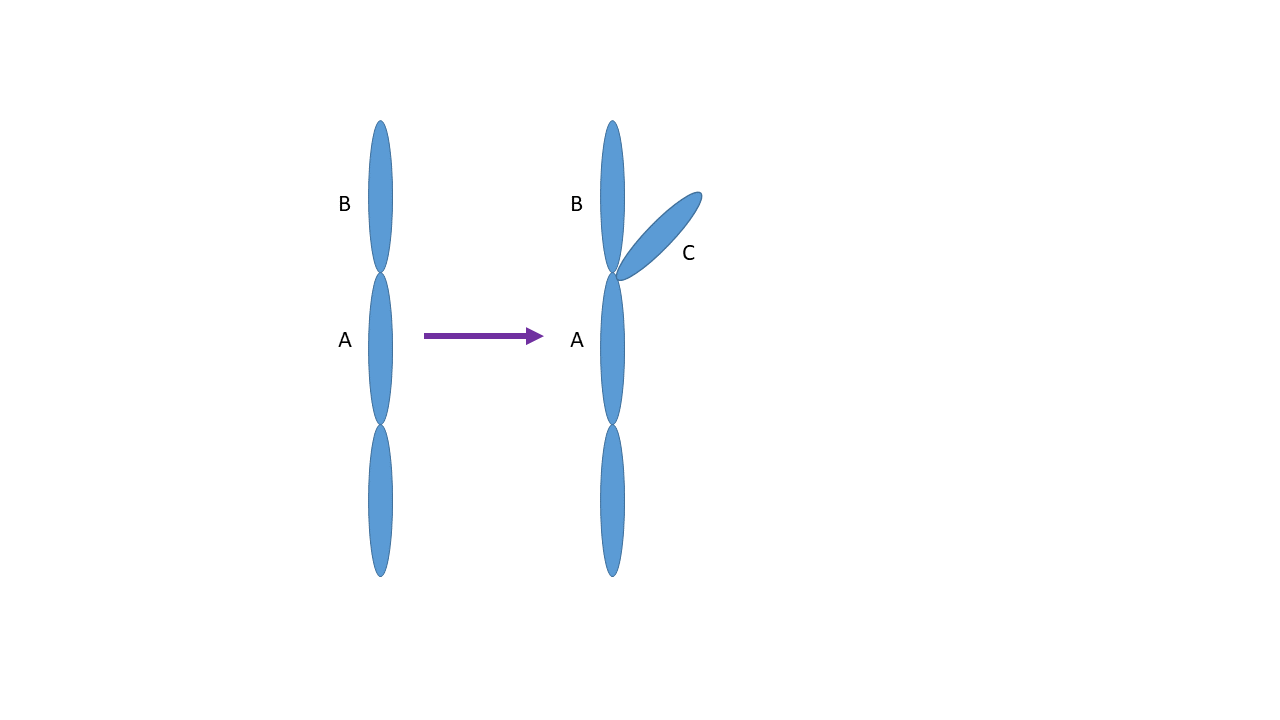
\includegraphics[width=4.0in,keepaspectratio=true]{side_branch}
\caption{\label{fig:side_branch} Schematic diagram of side branching}
\end{figure}

A typical loop over neighbors has the structure
\[
\sum_{i}\sum_{j\in Nghb(i)}
\]
The sum over $j$ may also have a restriction that the interaction is only evaluated
for $i<j$ to avoid duplicate interactions. The issue that arises, is that any
modifications that are identified in a loop over particles of this sort can only
be permanently applied to the particles indexed by $i$. The particles in the neighbor list
indexed by $j$ are copies of the original particle data, which may reside on other
processors, and changes made to the copies will disappear when the neighbor list is rebuilt.

To maintain and update the connectivity information, the following information is maintained
on each segment
\begin{list}{$\bullet$}{}
\item the number of segments that this segment is bonded to. The maximum number is 4.
\item a list of ids for the segments that are bonded to this segment (up to 4)
\item a list of cpus for the segments that are bonded to this segment (up to 4)
\item a list describing the site (1 or 2) at which the bonded segments are connected (up to 4)
\item an integer enumeration specifying whether a segment is a growth tip or not
\item a flag indicating that this segment is fusing to another segment
\item a flag indicating that this segment going to split in a fusion event
\item a flag indicating that this segment was created during a fusion event
\item the id of the segment that this particle is fusing to
\item the cpu of the segment that this particle is fusing to
\item a list of segment ids that were deleted from this segment (up to 2)
\item a list of segment cpus that were deleted from this segment (up to 2)
\end{list}
Each segment has a site at either end that is capabable of forming bonds with other segments.
These sites are labeled 1 and 2 and each site can be bonded to a maximum of two other segments
for a maximum of four bonds per segment. The last seven items in the list are only used to
support fusion of a growth tip to another segment. Not all of the parameters are necessarily
used simultaneously by all segments involved in the fusion event.

A major function of the simulation is maintaining these connectivities and it is complicated
to a significant degree by the behavior of the loops over neighbors. Generally, when new
segments are created, they are spawned from a parent segment. At the moment of creation,
the permanent copy of both the parent and the newly created child segment are available to
to the program and modifications to their data will be preserved. Thus, when a growth tip
generates a new tip or splits into two new tips, all the permanent information for both the
parent segment and the new segments are available and all bonding information can be updated
at the same time.

The situation is more complicated for side-branching from an interior segment. This
is illustrated in Figure \ref{fig:side_branch}. In the figure, the interior segment A is bonded
to segment B and a side branch forms in segment A at the end that is bonded to segment B. The
resulting segment C is bonded to both A and B. At the moment when segment C forms, both the
permanent data for A and C are available, but not the data for B. A can set its internal data
so that it is bonded to C and C, because it has access to A's internal data and can see that the
end bonded to C is also bonded to B, can set its
internal data so that it it is bonded to A and B. However, at this point B's bonding data does
not list C as a bonding partner.
This must be fixed up later when the loop to calculate forces is performed. Furthermore, to
guarantee that segment C's permanent data is modified, the restriction $i<j$ cannot be used.
Before evaluating the forces between a pair of segments, each segment in the pair
checks to see if it bonded to the other segment. If it is not, then it checks the bonding
information in the neighbor to see if the neighbor is bonded to it. If the neighbor is bonded
then the segment updates its bonding information to list the neighbor as a bond. In the case
of side branching, segment C is bonded to segment B but B is not bonded to segment C.
In the force loop, segment B will check the bonding information of segment C and find that
segment C lists B as a bonding partner. Based on this, segment B will update its bond
information to include C.

\begin{figure}
\centering
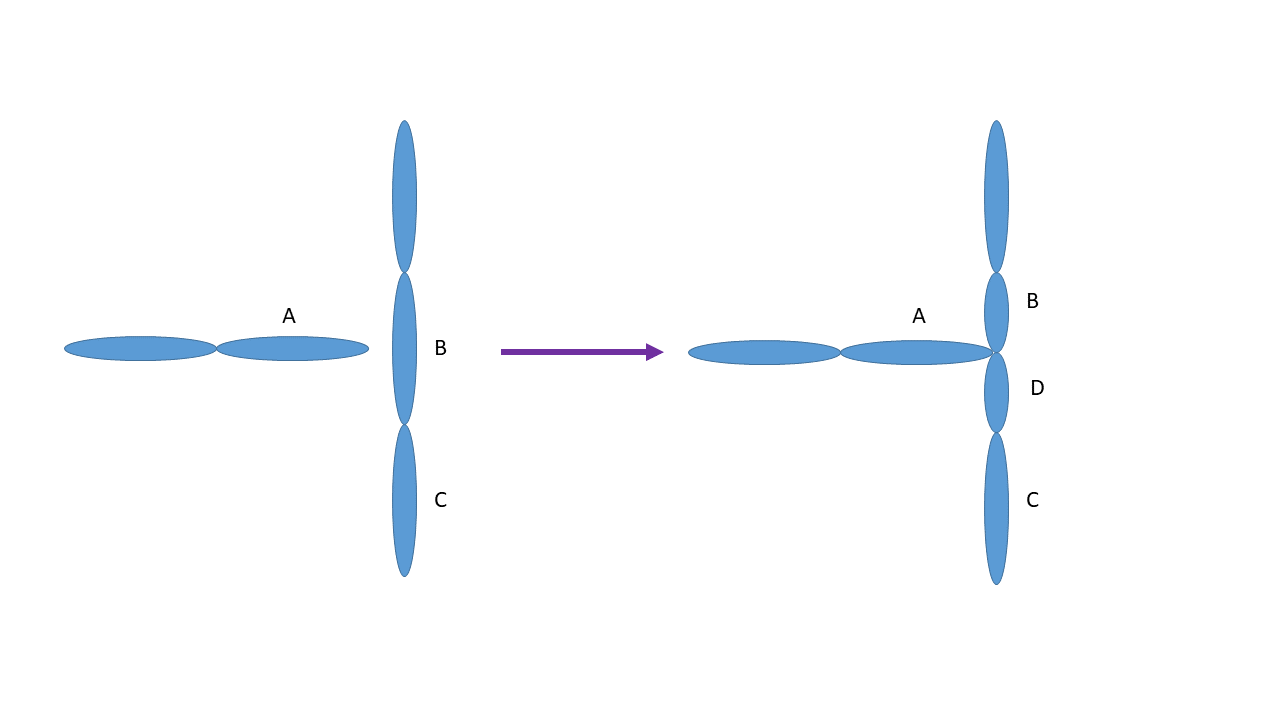
\includegraphics[width=4.0in,keepaspectratio=true]{fusion}
\caption{\label{fig:fusion} Schematic diagram of a growth tip fusing with an interior segment}
\end{figure}

Fusion of a growth tip with an interior segment requires the addition of several more loops
over neighbors in order to maintain an accurate record of connectivity. A schematic diagram
of a tip fusion event is shown in Figure \ref{fig:fusion}. When a tip fuses to another segment,
the other segment splits at the point where the fusion occurs and two new segments are formed.

Computationally, a tip fusion event occurs in four separate steps:
\begin{enumerate}
\item In a double loop over all segments and their neighbors, a tip identifies another segment
that it is going to fuse with. The tip labels itself as fusing and stores the id and cpu of the
fusing partner. In Figure \ref{fig:fusion} segment A identifies segment B as a fusion partner
and marks itself accordingly. Segment A also adds segment B to its list of bonding partners,
\item A second double loop over all segments and their neighbors is performed and each segment
checks its neighbors to see if it is a fusing tip and if it has marked the segment as a fusing
partner. If it finds that it is a fusing partner, the segment marks itself as splitting and
stores the id and cpu of the tip that it is fusing with. It also adds the tip as a bonding
partner,
\item A third loop over segments is performed and all segments marked for splitting are split
into two segments. In the example in Figure \ref{fig:fusion}, segment B generates segment D and
marks itself as having just split. Segment D is marked as being a new segment.
The split is done in a consisistent way so that the new segment is generated at the end of the
original segment corresponding to bonding site 2. Because of this, the bonds at site 2 on the
original segment B to segment C are no longer valid and need to be replaced with bonds to D.
Similarly, bonds to A, B and C can be added to D at this point since D has access to B's
connectivity data. However, A does not list D as a bonding partner and C needs to modify its
bonding data to remove the bonds to B and add bonds to D. To do this, B stores the ids and cpus
of the one or two bonds to C that were deleted.
\item A fourth double loop including neighbors is performed to fix up the bonds on segment C.
Bonds between segment A and D and segment C and D will get fixed in the force loop when
bonds are recognized between segments A and C and segment D. Segment B will still show up as
a neighbor of
segment C in the cleanup loop. However, segment B will be marked as having just been split and
will list a
bond to C as having been deleted. This is a signal to C to remove B as a bonding partner.
\end{enumerate}
Once these operations have been completed, the fusion flag, split flag and new segment flag are
all set to zero before the f

\section{Cylinder interactions}
Our model for interacting cylinders is based on the minimum distance between two
line segments. The segments are defined by the line joining the centers of the two
end caps for each cylinder. If these two points are defined as $\rvec_1$ and $\rvec_2$
and the separation between them is defined as $\rhvec = \rvec_2-\rvec_1$ then the line
segment $\Rvec(\tau)$ joining the endpoints is defined as
\[
\Rvec(\tau) = \rvec_1 +\tau\rhvec\;\;\;\;\;\;\;\mbox{for}\;\;\tau\in [0,1]
\]
For two cylinders $i$ and $j$ defined by the line segments $\Rvec_i(\tau_i)$ and
$\Rvec_j(\tau_j)$ we can find the minimum separation distance by minimizing
\begin{eqnarray*}
\chi & = & \left|\Rvec_i(\tau_i)-\Rvec_j(\tau_j)\right|^2 \\
     & = & \left|\rvec_{i1}-\rvec_{j1}\right|^2+2\tau_i(\rvec_{i1}-\rvec_{j1})\cdot\rhvec_i
          -2\tau_j(\rvec_{i1}-\rvec_{j1})\cdot\rhvec_j \\
     & + & \tau_i^2\left|\rhvec_i\right|^2 + \tau_j^2\left|\rhvec_j\right|^2
           - 2\tau_i\tau_j\rhvec_i\cdot\rhvec_j
\end{eqnarray*}
subject to the constraints $0\le\tau_i\le 1$ and $0\le\tau_j\le 1$.

Setting the gradients of $\chi$ with respect to $\tau_i$ and $\tau_j$ equal to
zero gives the coupled linear equations
\begin{eqnarray*}
-(\rvec_{i1}-\rvec_{j1})\cdot\rhvec_i & = & \tau_i\left|\rhvec_i\right|^2
                                        - \tau_j\rhvec_i\cdot\rhvec_j \\
(\rvec_{i1}-\rvec_{j1})\cdot\rhvec_j & = & - \tau_i\rhvec_i\cdot\rhvec_j
                                       + \tau_j\left|\rhvec_j\right|^2
\end{eqnarray*}
This can easily be solved in most cases for $\tau_i$ and $\tau_j$.
After a solution is found, it is necessary to check that the $\tau_i$ and $\tau_j$
satisfy the constraints. If they don't then the solution can be found by setting the
values of $\tau_i$ and $\tau_j$ to the limits 0 and 1 and optimizing the remaining
variable to find a minimum distance value. This may require and exhaustive search through
up to four values.

A corner case occurs when $\rhvec_i$ and $\rhvec_j$ are parallel. In this case the
determinant vanishes and there is no unique solution. An {\em ad hoc} solution can be
found by fixing $\tau_i$ to 0 and 1 and then minimizing $\tau_j$. Based on the values
of $\tau_j$, a pair of values can be chosen the represent the minimum distance between
the line segments.

The force between the two cylinders is some function $\Fvec(R)$ of the minimal
distance $R=|\Rvec_i(\tau_i)-\Rvec_j(\tau_j)|$ between the two cylinders. The
force must still be partitioned between the sites defining the cylinder. To do
this, we assume that $F(R)$ is generated from a potential $U(R)$. The force is
then
\[
\nabla_{\Rvec}U(R) = \Fvec(R)
\]
If we write $\Rvec_j(\tau_j)$ as
\[
\Rvec_i(\tau_i) = \rvec_i + \tau_i (\rvec_{i2}-\rvec_{i1})
\]
then the gradient of $U(R)$ with respect to $\rvec_{i1}$ is
\begin{eqnarray*}
\nabla_{\rvec_{i1}}U(R) & = & \frac{\partial U}{\partial R}\nabla_{\rvec_{i1}}R\
 = \frac{\partial U}{\partial R}\frac{\Rvec}{R} (1-\tau_i)
\end{eqnarray*}
Identifying $-\partial U/\partial R$ as some function $F(R)$ gives the final
relation
\[
\fvec_{i1} = F(R)\frac{\Rvec}{R}(1-\tau_i)
\]
for the force acting on site 1 of segment $i$. The force acting on site 2 of segment
$i$ is just
\[
\fvec_{i2} = F(R)\frac{\Rvec}{R}\tau_j
\]
The expressions for the forces on the two sites of segment $j$ are similar.
\bibliographystyle{unsrt}
\bibliography{bmx}
\end{document}
